% Chapter Template

\chapter{Pile Up Studies} % Main chapter title

\label{Chapter 8} % Change X to a consecutive number; for referencing this chapter elsewhere, use \ref{ChapterX}

\lhead{Chapter 78 \emph{PU Studies}} % Change X to a consecutive number; this is for the header on each page - perhaps a shortened title

%----------------------------------------------------------------------------------------
%	SECTION 1
%----------------------------------------------------------------------------------------

\section{Jet}
\subsection{Efficiencies}
In order to test the jet finding algorithm the first study that must be undertaken is into the matching efficiency of the L1 jets to the generator level quantities for a ttbar(PU 40, $\tau_b=50ns$) MC sample. The gen jets are made by running the anti-kt 4 algorithm **REF** on the generator level quantities. The gen jet is said to be matched if within ${\Delta R}^2<33$ of a L1 jet (the greatest extent of the L1 jet). The matching efficiency for alljets and the 4 jet is shown in figure \ref{match}. It can be seen that the efficiency after PUS/seed drops at low $p_T$, however, for the trigger such jets are mainly relevant for $H_T$ which is shown to perform well. Inefficiencies at high $p_T$ are caused by the 'chain veto', however, the jet algorithm guarantees there is always a comparable or higher jet in the event in such cases. The performance compared to GCT is seen to be greatly improved.  
\begin{figure}
\hfill
\subfigure[All jets\label{fig:label:alljet}]{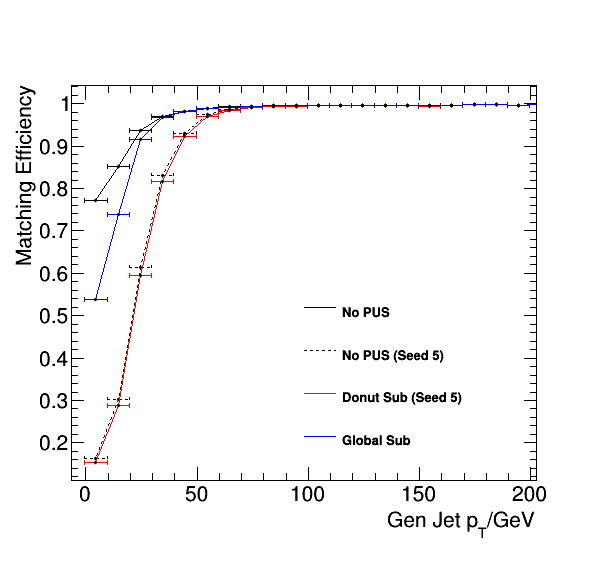
\includegraphics[width=7cm]{Figures/alljet}}
\hfill
\subfigure[4th jet\label{fig:label:jet4}]{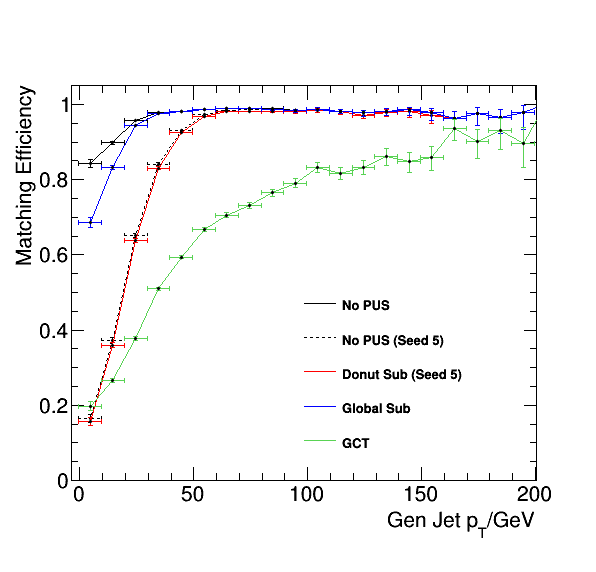
\includegraphics[width=7cm]{Figures/jet4}}
\hfill
\caption{Matching efficiencies for jets showing effect of seed and PUS at low energies. In \ref{fig:label:jet4} a comparison with the GCT is shown.}
\label{match}
\end{figure}
\subsection{Calibration}
The energy of the L1 jets must be calibrated using generator level quantities. The scheme for calibration is outlined in \cite{l1jet_calibration}. Essentially, using a QCD PU 40, 50ns sample, the resolution (defined as $p^{L1}_{T}/p^{gen}_{T}$) and $p^{L1}_{T}$ are plotted against $p^{gen}_{T}$ and fitted. The fits are then plotted against each other giving calibration factors as a function of $p^{L1}_{T}$. The calibration is carried out in bins of $\eta$ to account for the difference in performance of the detector. Where the matching efficiency is low it is not possible to fit and so the calibration has a lower bound on $p_T$. This was found to occur at $20GeV$. The calibration factors change depending on the PUS regime.    
\begin{figure}
\hfill
\subfigure[All jets\label{fig:label:alljet}]{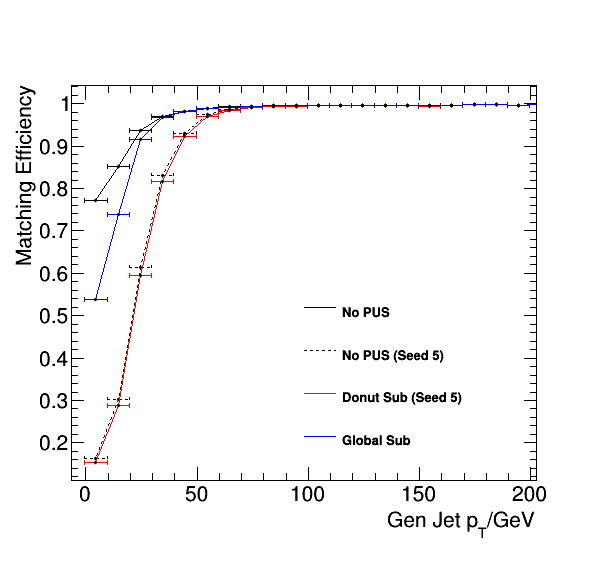
\includegraphics[width=7cm]{Figures/alljet}}
\hfill
\subfigure[4th jet\label{fig:label:jet4}]{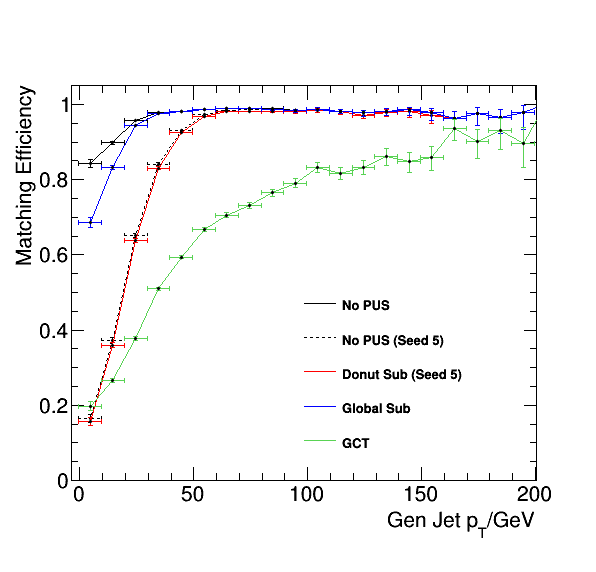
\includegraphics[width=7cm]{Figures/jet4}}
\hfill
\caption{Resolution before and after calibration. In \ref{fig:label:jet4} a comparison with the GCT is shown.}
\label{match}
\end{figure}
\section{PUS Testing}
\subsection{Reso}
In this section plots are shown for the highest $|\eta|$ bin as the detector perofrmance is expected to worsen with larger $|\eta|$ and so PUS will have the largest effect. The first test of any PUS scheme is the effect on the resolution. In an ideal post PUS scenario this will be flat as a function of NVTX. In figure \ref{fig:label:resolution1} this is plotted for a particular $p^{gen}_T$ and $\eta$ bin. It can be seen that the response flattens for both PUS regimes. This is summarised in \ref{fig:label:resolution2} where the gradient from the fit to the resolution plot is shown to reduce after PUS for a range of $p^{gen}_T bins$.  
\begin{figure}
\hfill
\subfigure[All jets\label{fig:label:resolution1}]{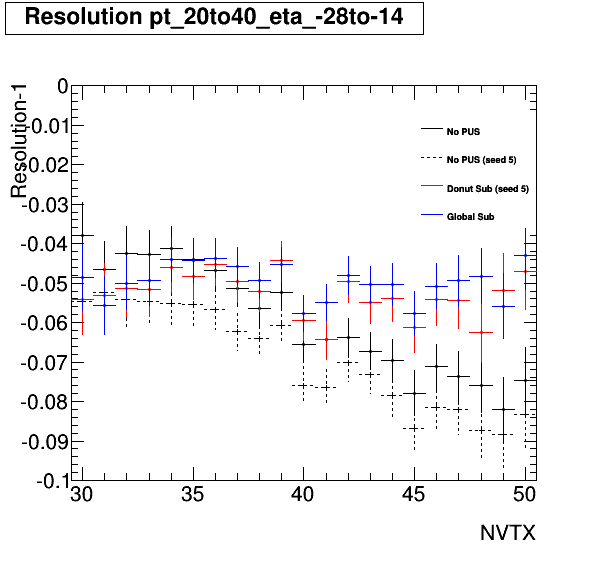
\includegraphics[width=7cm]{Figures/pt_20to40_eta_-28to-14}}
\hfill
\subfigure[All jets\label{fig:label:resolution2}]{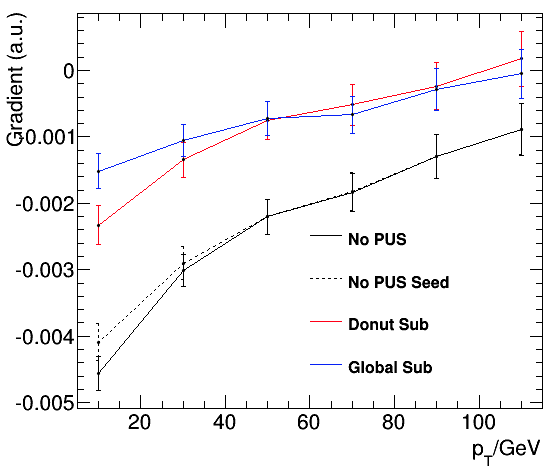
\includegraphics[width=7cm]{Figures/p1eta_14to28_calib_fits}}
\caption{In \ref{fig:label:resolution1} response versus NVTX is shown for a particular eta bin showing the response flattens after PUS. In \ref{fig:label:resolution2} the fit gradient for the response against NVTX for different $p_{T}$ bins is shown.}
\label{fig:label:resolution}
\end{figure}
\subsection{Rates}
The rate/efficiency is defined as the proportion of jets for signal/background passing a particular $p_{T}$ cut. For the trigger the key test is to see that the efficiency for signal may be maintained while reducing the background rate. Neutrino gun (PU40, 50ns) and ttbar (PU40, 50ns) samples were used as background and signal. In figure \ref{fig:label:rateeff} the rate versus efficiency is plotted for the 4th jet. This shows PUS reducing the rate while maintaining efficiency. Performance compared to the GCT is shown to be greatly improved. In \ref{fig:label:rates} a particular cut on pt (30GeV) is chosen and the dependence on the NVTX is shown. PUS greatly reduces the rate and as shown in \ref{fig:label:ratenvtxt} maintains the efficiency near the gen level (0.74).
\begin{figure}
\centering
    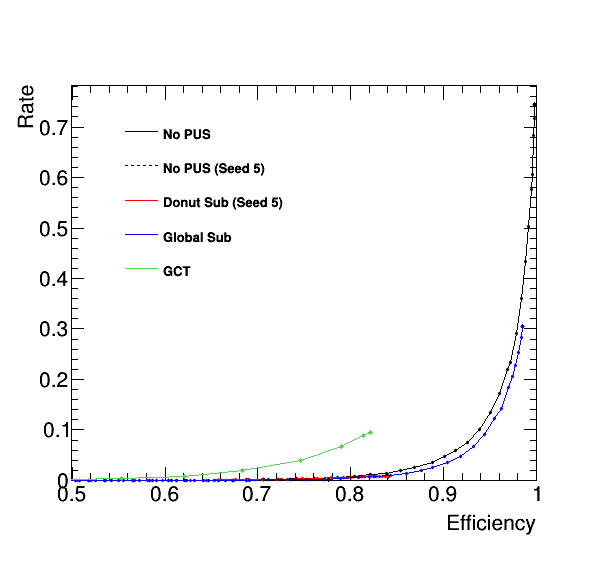
\includegraphics[width=0.8\textwidth]{Figures/rateeffjet4}
  \caption{Rate of a background (neutrino) sample against efficiency from a ttbar sample showing improvement after PUS.}
  \label{rateff}
\end{figure}
\begin{figure}
\hfill
\subfigure[Rate Jet 4\label{fig:label:ratenvtxn}]{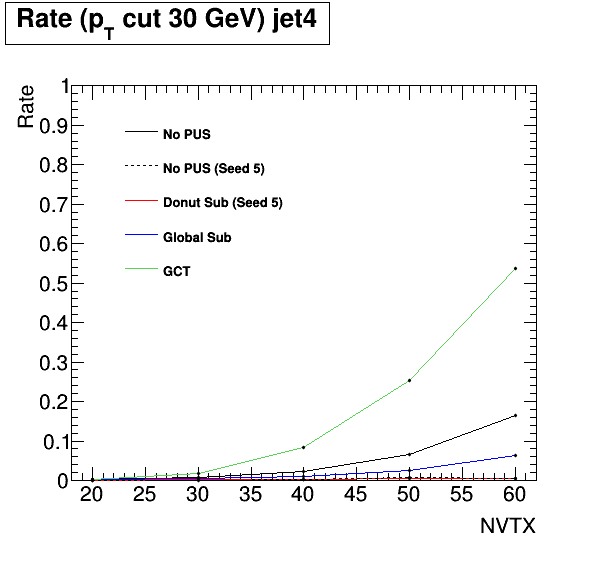
\includegraphics[width=7cm]{Figures/neutrinojet4}}
\hfill
\subfigure[Eff Jet 4\label{fig:label:ratenvtxt}]{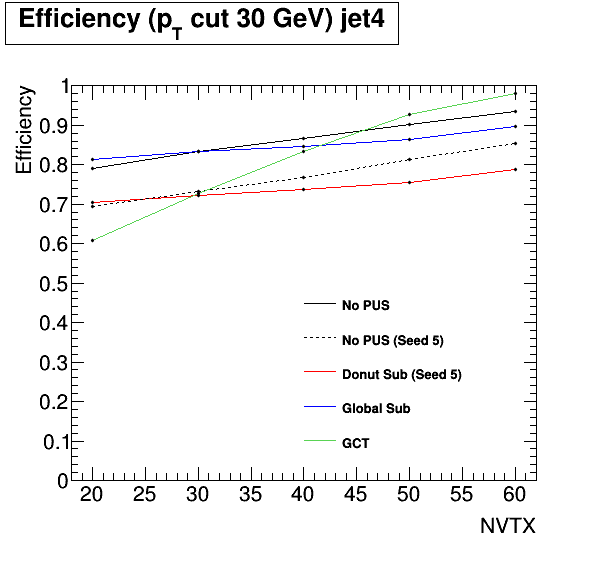
\includegraphics[width=7cm]{Figures/ttbarjet4}}
\centering
\subfigure[Rate vs Eff\label{fig:label:rateeff}]{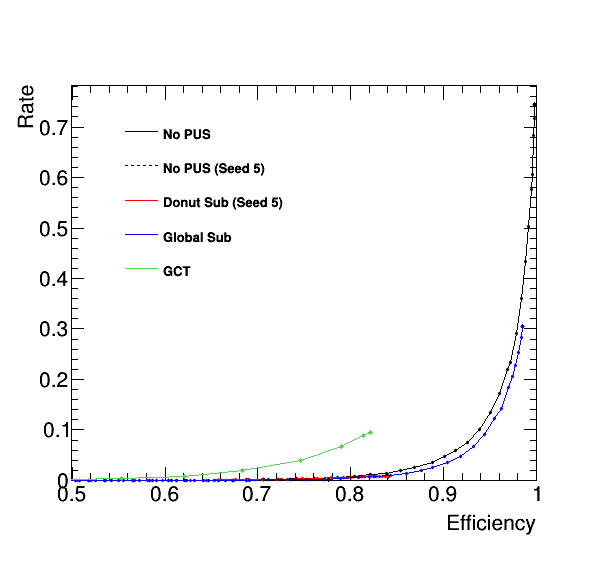
\includegraphics[width=7cm]{Figures/rateeffjet4}}
\caption{In \ref{fig:label:rateeff} the optimisation of the rate is shown versus the efficiency. The dependence of the rates and efficiency for $p_T > 30 GeV$ on the NVTX is shown in figure \ref{fig:label:ratenvtxn} and \ref{fig:label:ratenvtxt}. The gen efficiency for \ref{fig:label:ratenvtxt} is 0.74.}
\label{fig:label:rates}
\end{figure}
\subsection{Turn On Plots}

To benchmark the performance of the L1 jets their $p_T$ must be compared with matched generator level quantities. To do this the generator level quantity is plotted with a cut on the matched L1 quantity (the turn on). This is shown for two representative examples in figure \ref{turnon}. As can be seen the turn on for the GCT is less sharp than that for the stage 2 quantities. This shows better agreement with gen for the upgraded system.
\begin{figure}
\centering
    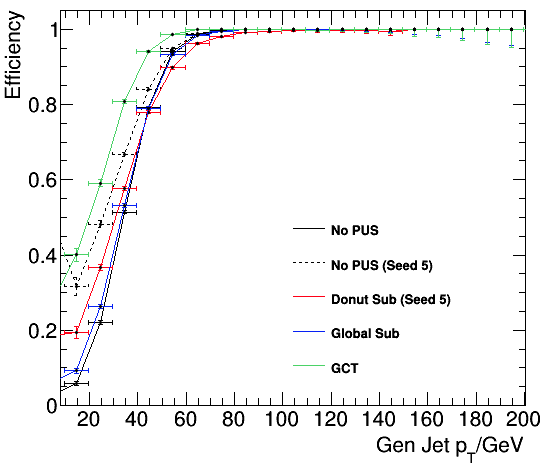
\includegraphics[width=0.8\textwidth]{Figures/jet4_40}
  \caption{Turn on curve at 40 GeV showing comparable behaviour for the phase 2 quantities and a much shallower turn on for GCT.}
  \label{turnon}
\end{figure}
\subsection{Energy Sums}

Lastly the energy sums which are used to make triggers based $H_T$ and $\cancel{H_T}$ were investigated. To nullify the problem of not having calibration below $20GeV$ only jets above this are included in the sums.  As PU is uniform it should not affect the missing energy in the event. The result for $H_T$ and $\cancel{H_T}$ for a ttbar sample are shown in figure \ref{sums}. PUS improves the agreement as compared to gen.  The $H_T$ shows especially good agreement with gen for the case of a seed as compared to global. This is due to the under-subtraction bias of the global rho method. The $\cancel{H_T}$ shows similar levels of agreement for all cases as expected. 
\begin{figure}
\hfill
\subfigure[$H_T$\label{fig:label:ht}]{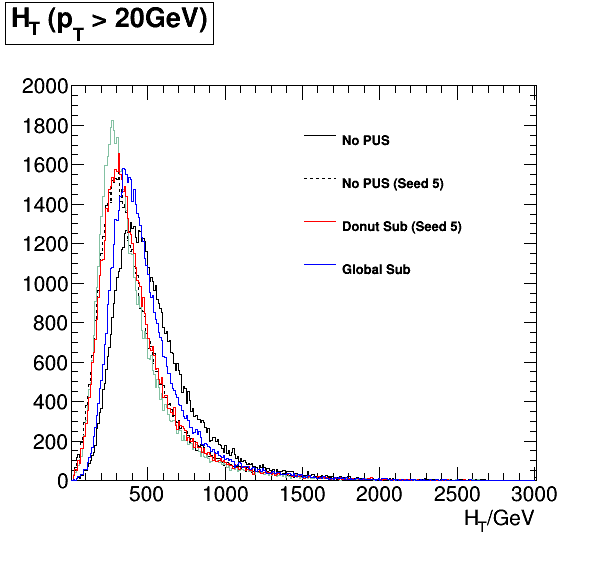
\includegraphics[width=7cm]{Figures/ht_ttbar}}
\hfill
\subfigure[$\cancel{H_T}$\label{fig:label:mht}]{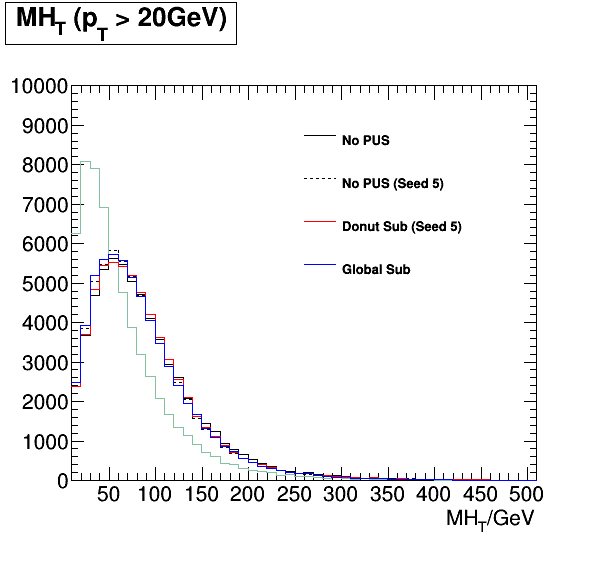
\includegraphics[width=7cm]{Figures/mht_ttbar}}
\caption{In figure \ref{fig:label:ht} the total energy shows good agreement with the generator level quantity. This is improved by requiring a seed threshold. In figure \ref{fig:label:mht} similar agreement is shown for all cases}
\label{fig:label:sums}
\end{figure}
\section{Conclusions}
The jet algorithm has been shown to function well, giving very compatible results with the offline anti-kT algorithm\footnote{$9\times9$ trigger tower corresponds to anti kt with $R =0.4$} and maintaining a high matching efficiency to generator level quantities. The PUS studies have shown that PUS is required for run 2. While both global and donut subtraction have been shown to flatten the response (\ref{fig:label:resolution} each has weaknesses that must be addressed. Figure \ref{fig:label:rateeff} shows that applying a seed threshold is comparable to global subtraction at killing rate while maintaining efficiency. Donut subtraction is shown to perform less well than applying the seed threshold alone. This is due to the susceptibility of donut subtraction to fluctuations. Further studies are underway to increase the sampling area for donut subtraction to reduce this issue. Figure \ref{fig:label:sums} shows global $\rho$ under-performing for the $H_T$. This is due to the under-subtraction bias leading to more energy being left in the event. This may be correcting by applying a seed threshold as for donut but calculating $\rho$ using all jets. 

Further studies are currently underway to utilise the $\eta$ dependence of the pileup.  The seed threshold applied may be altered depending on the location of the tower to further reduce rate in areas of high pileup while maintaining efficiency in low pileup regions. Improving calibrations such that lower energy jets may be utilised ( the current limit is 20GeV) is also key. Finally, increasing the sample size to use $3\times3$ towers for the seed should improve discrimination between pileup and boosted jets. 

    
